\documentclass[12pt,twoside]{report}
\usepackage{graphicx}
\usepackage{alphalph}
\usepackage{subcaption}
\usepackage[a5paper,margin=1cm]{geometry}
\renewcommand*{\thesubfigure}{(\arabic{subfigure})}
\begin{document}
\begin{figure}
\centering
\begin{subfigure}[b]{0.20\textwidth}
\centering
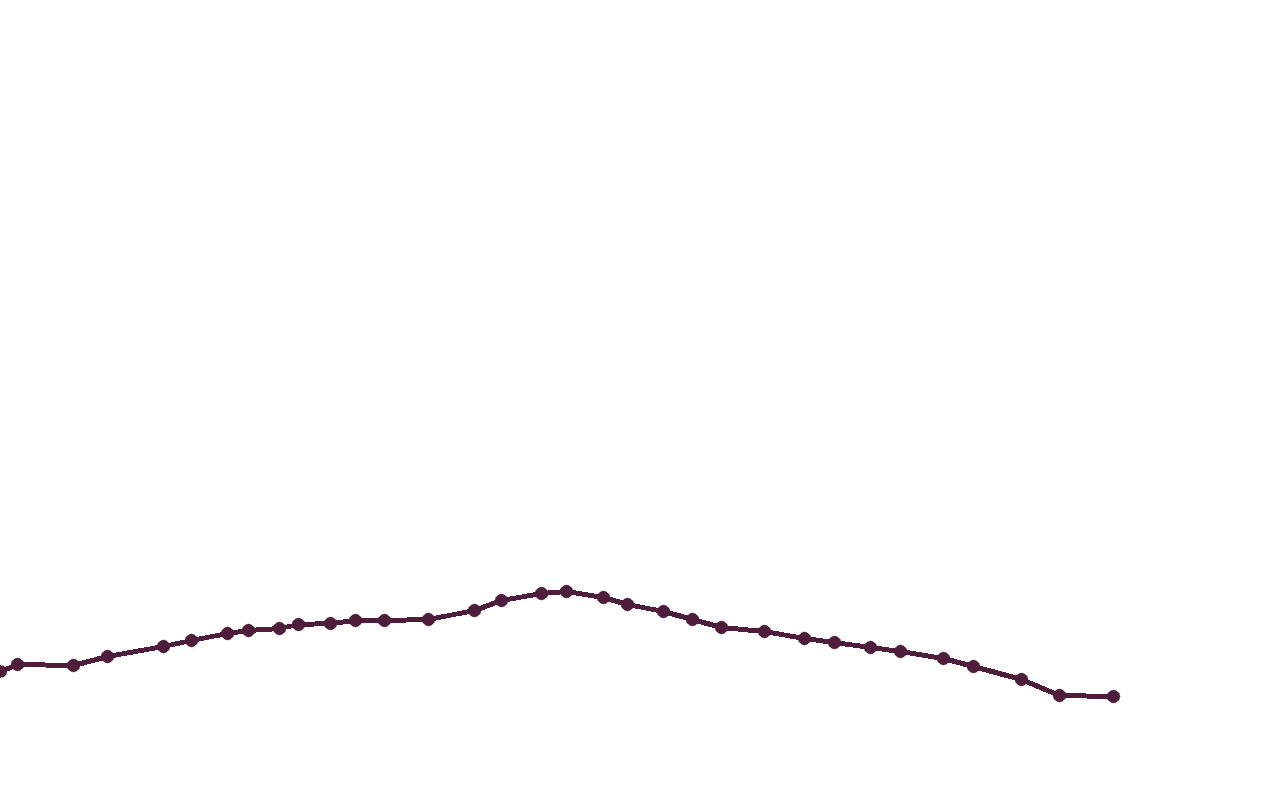
\includegraphics[width=\textwidth]{../../trajectories/50.png}
\caption{Id:50}
\end{subfigure}
\begin{subfigure}[b]{0.20\textwidth}
\centering
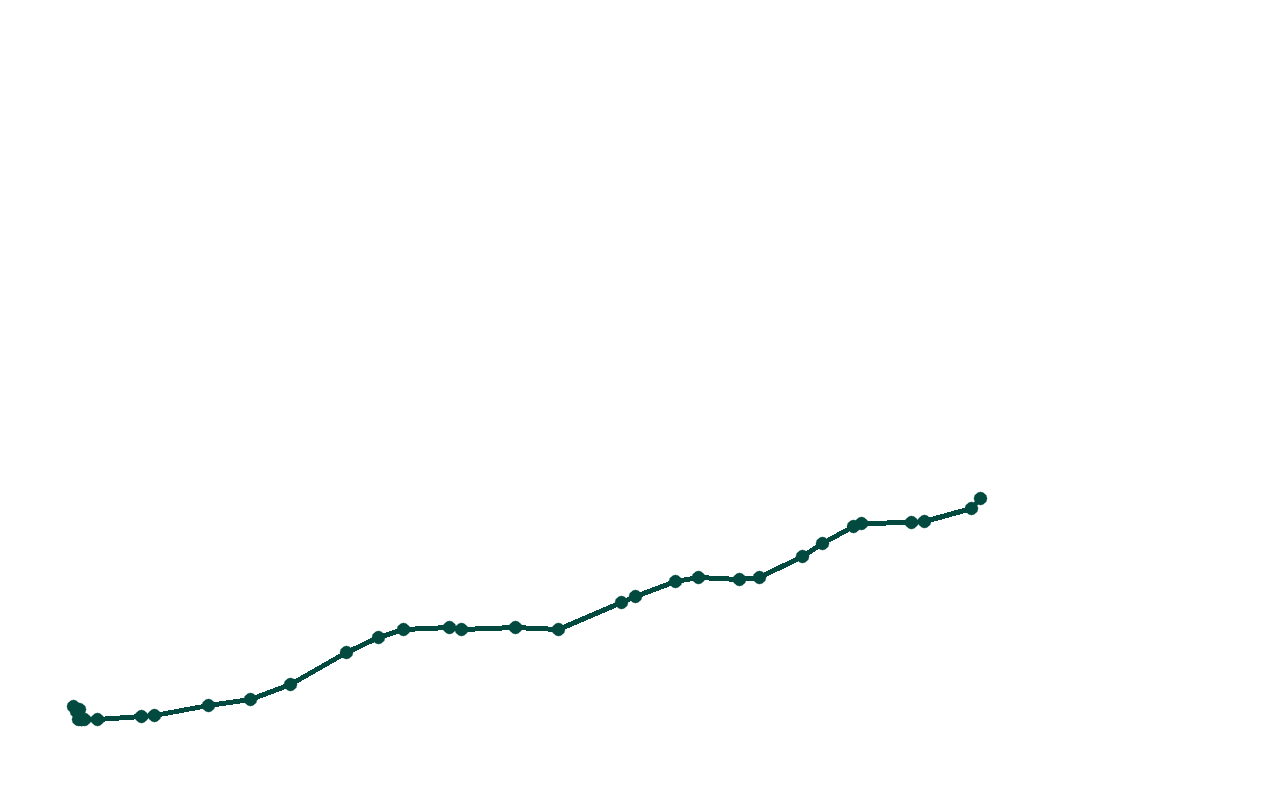
\includegraphics[width=\textwidth]{../../trajectories/136.png}
\caption{Id:136}
\end{subfigure}
\begin{subfigure}[b]{0.20\textwidth}
\centering
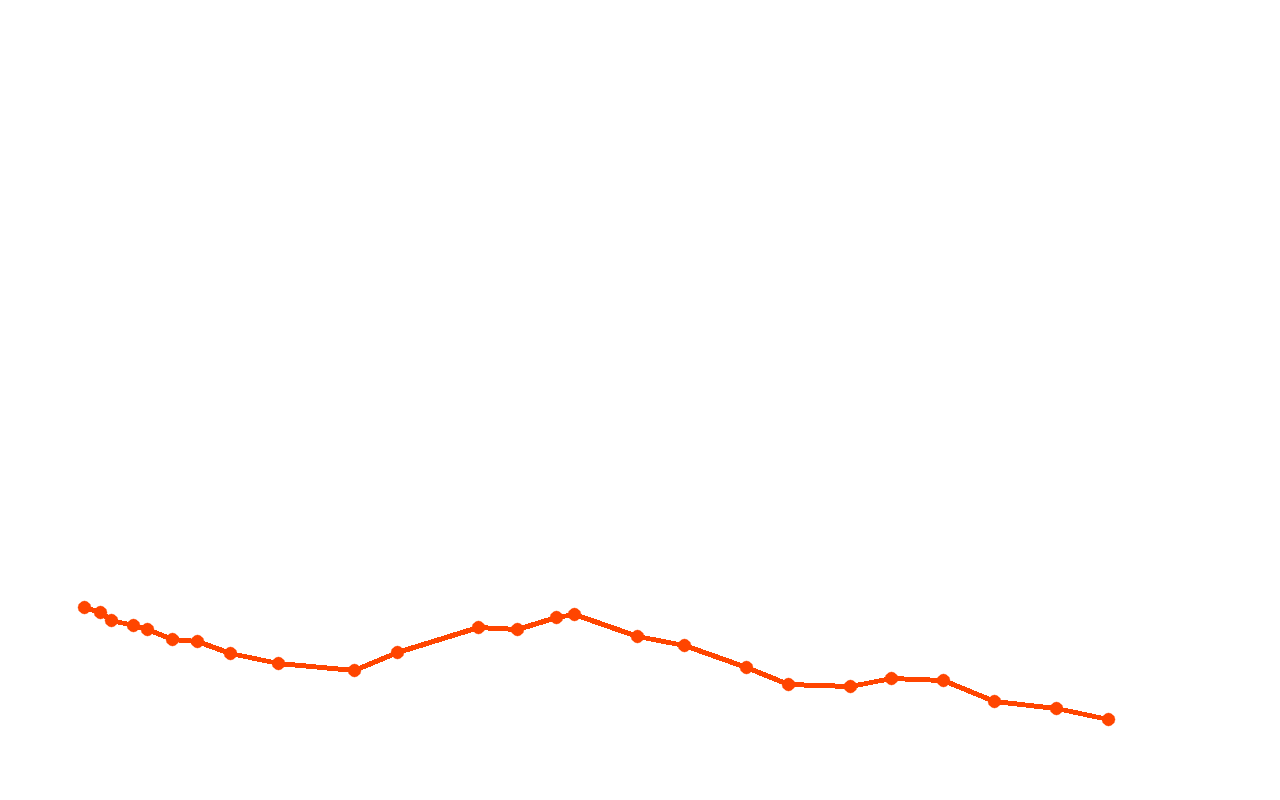
\includegraphics[width=\textwidth]{../../trajectories/188.png}
\caption{Id:188}
\end{subfigure}
\begin{subfigure}[b]{0.20\textwidth}
\centering
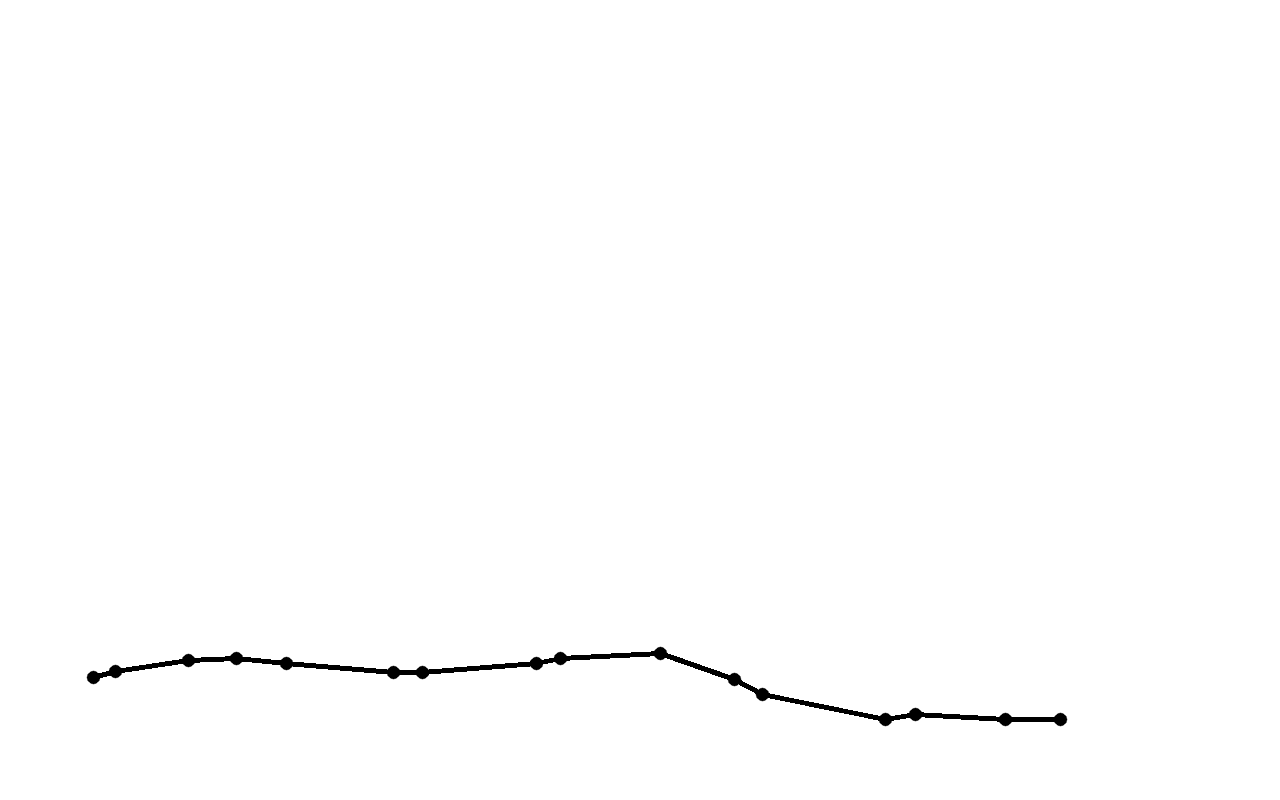
\includegraphics[width=\textwidth]{../../trajectories/252.png}
\caption{Id:252}
\end{subfigure}
\begin{subfigure}[b]{0.20\textwidth}
\centering
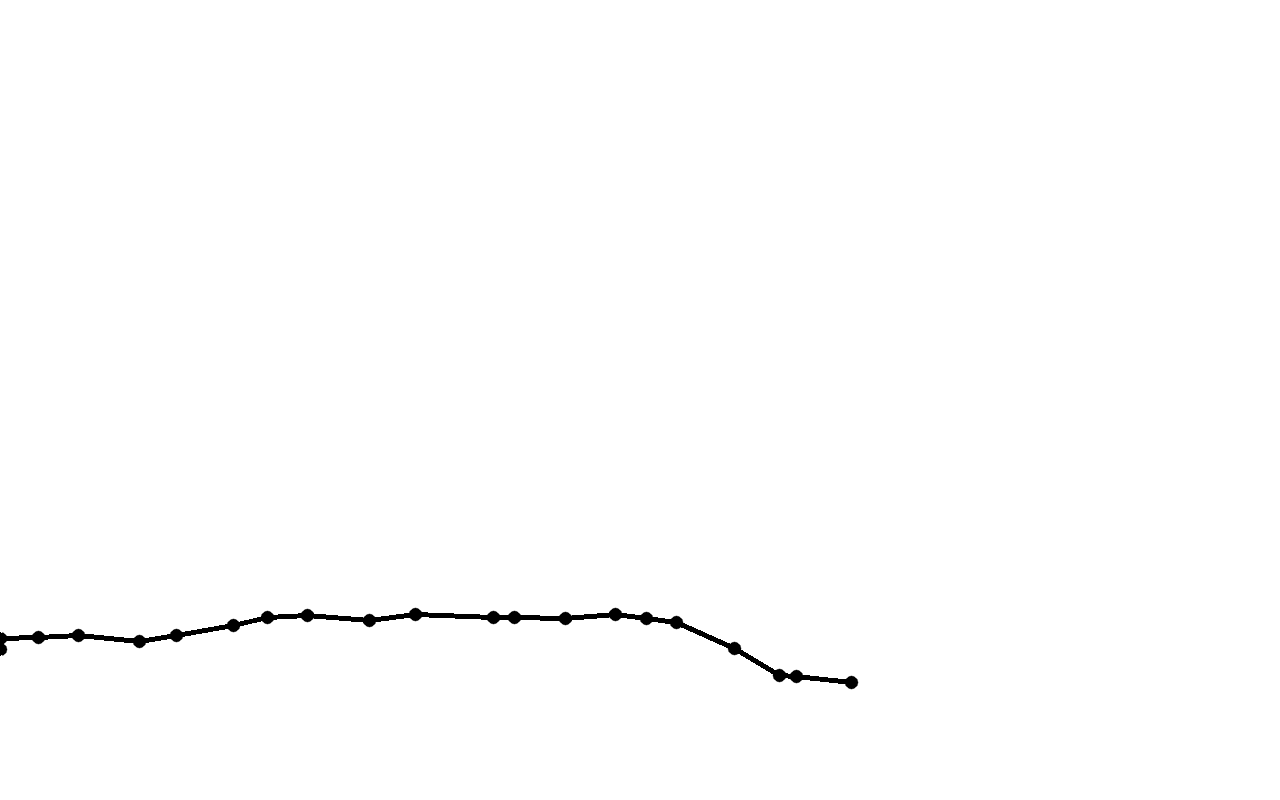
\includegraphics[width=\textwidth]{../../trajectories/490.png}
\caption{Id:490}
\end{subfigure}
\begin{subfigure}[b]{0.20\textwidth}
\centering
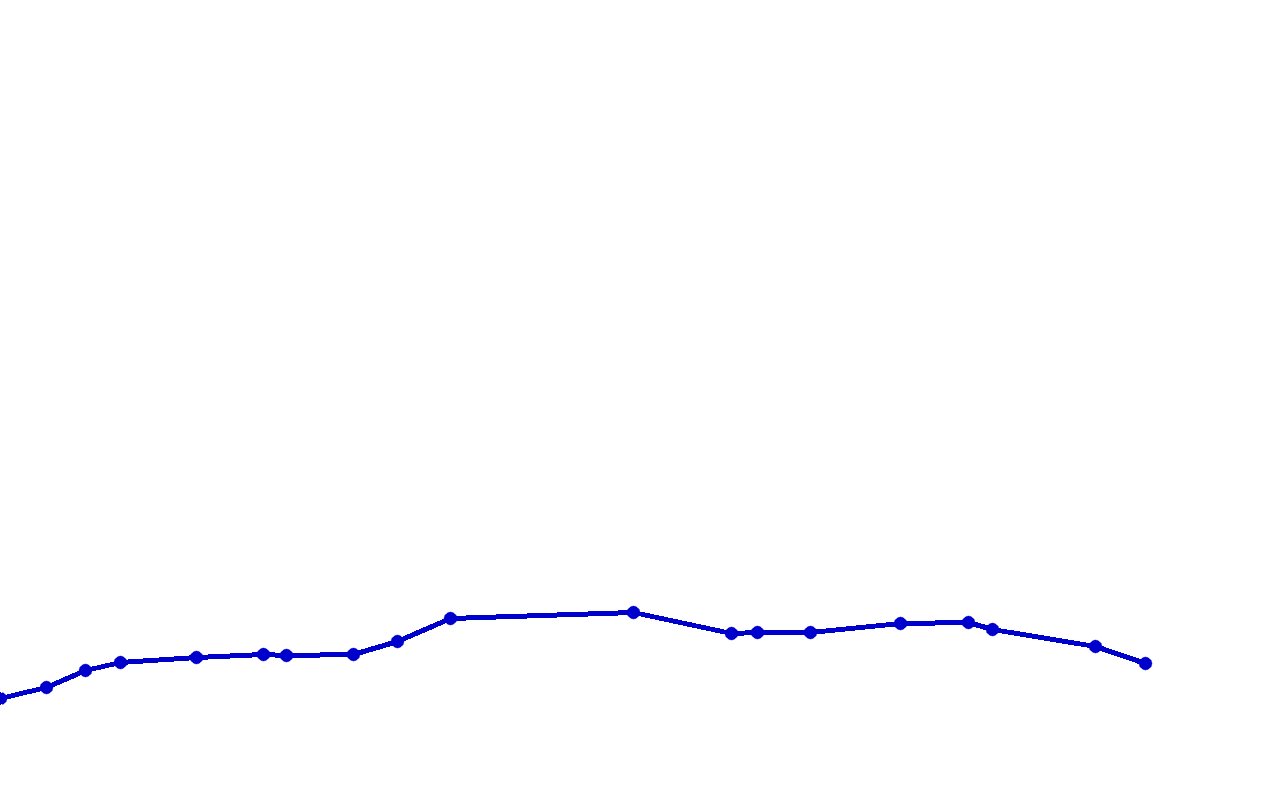
\includegraphics[width=\textwidth]{../../trajectories/889.png}
\caption{Id:889}
\end{subfigure}
\end{figure}
\end{document}